\section{src/main.cpp File Reference}
\label{main_8cpp}\index{src/main.cpp@{src/main.cpp}}
{\tt \#include \char`\"{}main.hpp\char`\"{}}\par


Include dependency graph for main.cpp:\begin{figure}[H]
\begin{center}
\leavevmode
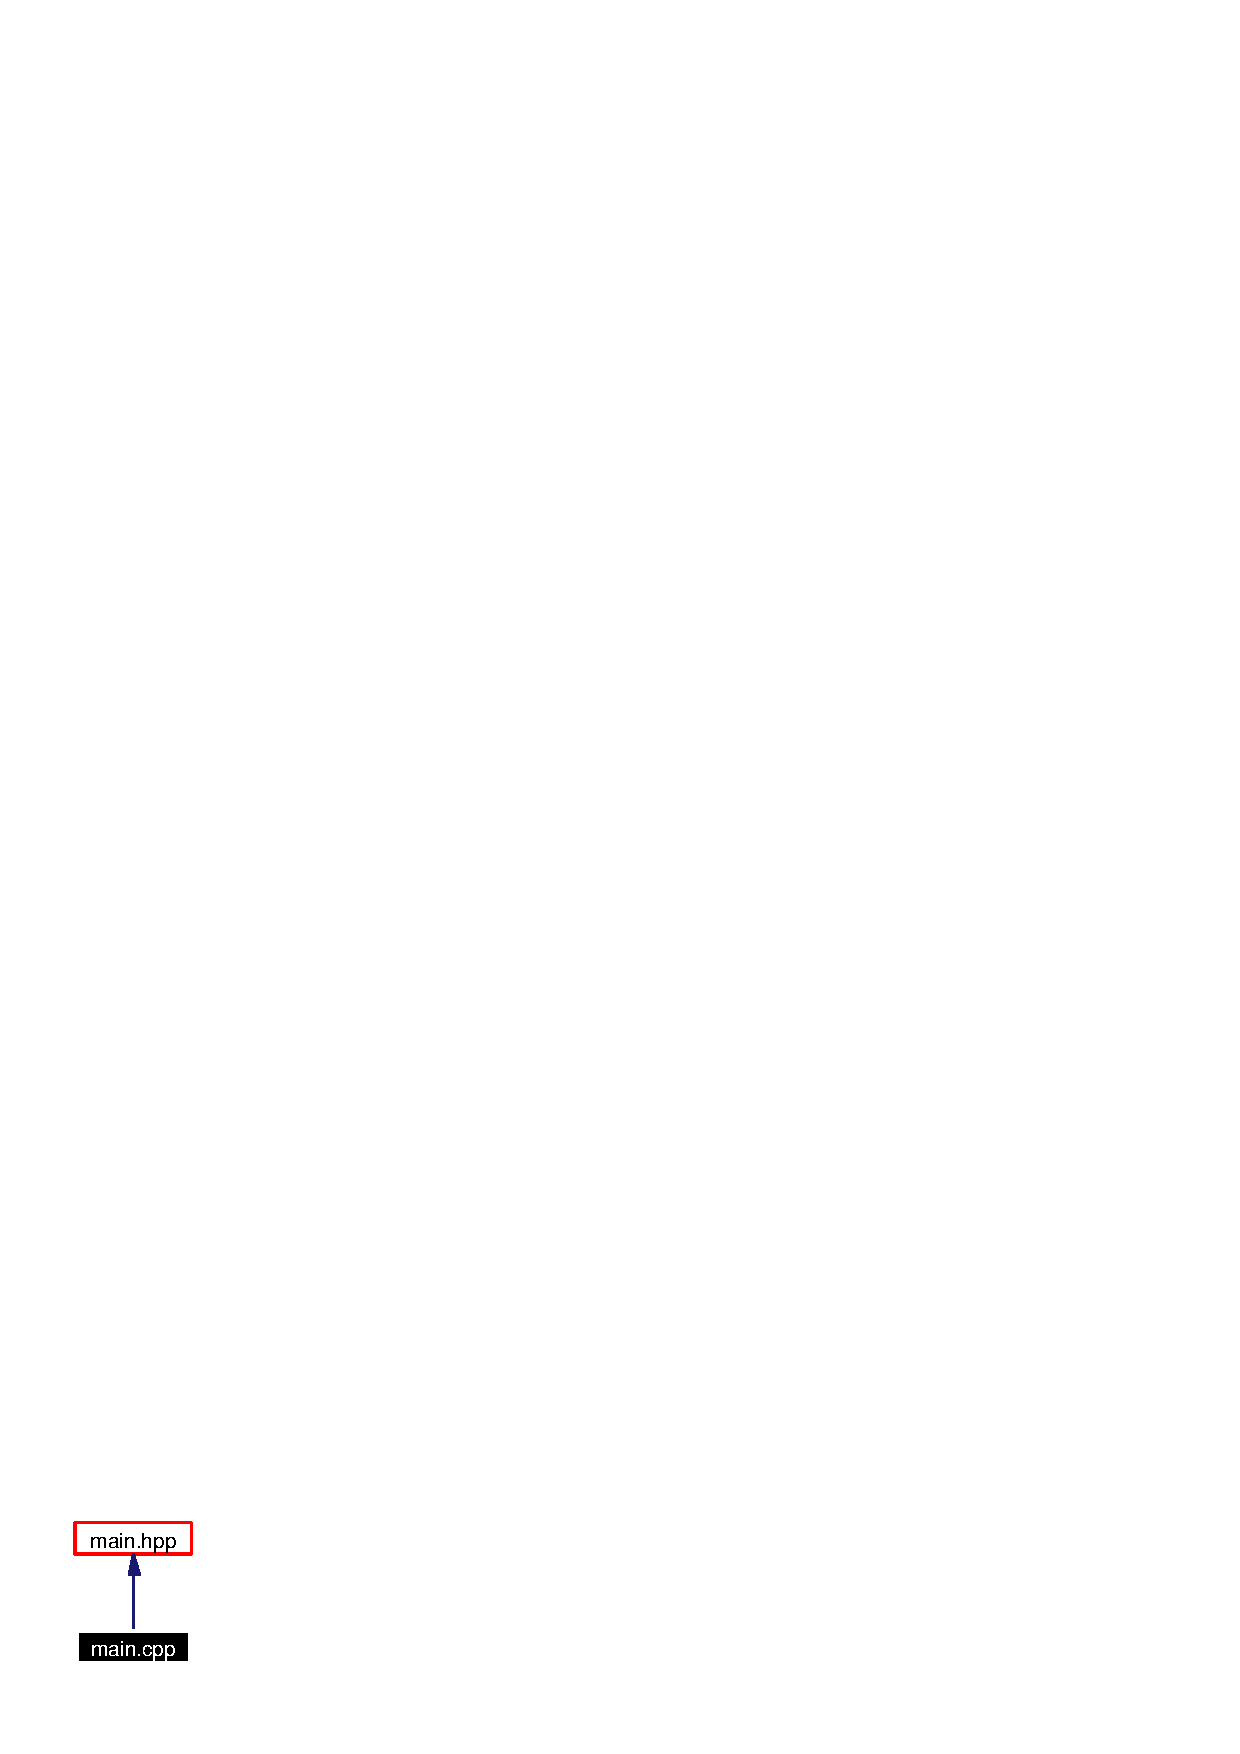
\includegraphics[width=46pt]{main_8cpp__incl}
\end{center}
\end{figure}
\subsection*{Functions}
\begin{CompactItemize}
\item 
int {\bf sdl\_\-start} ({\bf Log\-Engine} \&log)
\item 
void {\bf sdl\_\-stop} (void)
\item 
void {\bf run\-Gui\-Loop} ({\bf World\-Data} \&world\-Data, {\bf System\-Data} \&system\-Data, {\bf Log\-Engine} \&log, {\bf Data\-Engine} \&data, {\bf Input\-Engine} \&input, {\bf Graphics\-Engine} \&graphics, {\bf Physics\-Engine} \&physics, {\bf Gui\-Engine} \&gui)
\item 
void {\bf run\-Sim\-Loop} ({\bf World\-Data} \&world\-Data, {\bf System\-Data} \&system\-Data, {\bf Log\-Engine} \&log, {\bf Data\-Engine} \&data, {\bf Input\-Engine} \&input, {\bf Graphics\-Engine} \&graphics, {\bf Physics\-Engine} \&physics, {\bf Gui\-Engine} \&gui)
\item 
void {\bf initialize\-Sim\-Loop} ({\bf World\-Data} \&world\-Data, {\bf System\-Data} \&system\-Data, {\bf Log\-Engine} \&log, {\bf Data\-Engine} \&data, {\bf Input\-Engine} \&input, {\bf Graphics\-Engine} \&graphics, {\bf Physics\-Engine} \&physics, {\bf Gui\-Engine} \&gui)
\item 
void {\bf shutdown\-Sim\-Loop} ({\bf World\-Data} \&world\-Data, {\bf System\-Data} \&system\-Data, {\bf Log\-Engine} \&log, {\bf Data\-Engine} \&data, {\bf Input\-Engine} \&input, {\bf Graphics\-Engine} \&graphics, {\bf Physics\-Engine} \&physics, {\bf Gui\-Engine} \&gui)
\item 
void {\bf initialize\-Gui\-Loop} ({\bf World\-Data} \&world\-Data, {\bf System\-Data} \&system\-Data, {\bf Log\-Engine} \&log, {\bf Data\-Engine} \&data, {\bf Input\-Engine} \&input, {\bf Graphics\-Engine} \&graphics, {\bf Physics\-Engine} \&physics, {\bf Gui\-Engine} \&gui)
\item 
void {\bf shutdown\-Gui\-Loop} ({\bf World\-Data} \&world\-Data, {\bf System\-Data} \&system\-Data, {\bf Log\-Engine} \&log, {\bf Data\-Engine} \&data, {\bf Input\-Engine} \&input, {\bf Graphics\-Engine} \&graphics, {\bf Physics\-Engine} \&physics, {\bf Gui\-Engine} \&gui)
\item 
void {\bf initialize\-Main\-Loop} ({\bf World\-Data} \&world\-Data, {\bf System\-Data} \&system\-Data, {\bf Log\-Engine} \&log, {\bf Data\-Engine} \&data, {\bf Input\-Engine} \&input, {\bf Graphics\-Engine} \&graphics, {\bf Physics\-Engine} \&physics, {\bf Gui\-Engine} \&gui)
\item 
void {\bf shutdown\-Main\-Loop} ({\bf World\-Data} \&world\-Data, {\bf System\-Data} \&system\-Data, {\bf Log\-Engine} \&log, {\bf Data\-Engine} \&data, {\bf Input\-Engine} \&input, {\bf Graphics\-Engine} \&graphics, {\bf Physics\-Engine} \&physics, {\bf Gui\-Engine} \&gui)
\item 
int {\bf main} (int argc, char $\ast$$\ast$argv)
\end{CompactItemize}


\subsection{Function Documentation}
\index{main.cpp@{main.cpp}!initializeGuiLoop@{initializeGuiLoop}}
\index{initializeGuiLoop@{initializeGuiLoop}!main.cpp@{main.cpp}}
\subsubsection{\setlength{\rightskip}{0pt plus 5cm}void initialize\-Gui\-Loop ({\bf World\-Data} \& {\em world\-Data}, {\bf System\-Data} \& {\em system\-Data}, {\bf Log\-Engine} \& {\em log}, {\bf Data\-Engine} \& {\em data}, {\bf Input\-Engine} \& {\em input}, {\bf Graphics\-Engine} \& {\em graphics}, {\bf Physics\-Engine} \& {\em physics}, {\bf Gui\-Engine} \& {\em gui})}\label{main_8cpp_a6}


\index{main.cpp@{main.cpp}!initializeMainLoop@{initializeMainLoop}}
\index{initializeMainLoop@{initializeMainLoop}!main.cpp@{main.cpp}}
\subsubsection{\setlength{\rightskip}{0pt plus 5cm}void initialize\-Main\-Loop ({\bf World\-Data} \& {\em world\-Data}, {\bf System\-Data} \& {\em system\-Data}, {\bf Log\-Engine} \& {\em log}, {\bf Data\-Engine} \& {\em data}, {\bf Input\-Engine} \& {\em input}, {\bf Graphics\-Engine} \& {\em graphics}, {\bf Physics\-Engine} \& {\em physics}, {\bf Gui\-Engine} \& {\em gui})}\label{main_8cpp_a8}


\index{main.cpp@{main.cpp}!initializeSimLoop@{initializeSimLoop}}
\index{initializeSimLoop@{initializeSimLoop}!main.cpp@{main.cpp}}
\subsubsection{\setlength{\rightskip}{0pt plus 5cm}void initialize\-Sim\-Loop ({\bf World\-Data} \& {\em world\-Data}, {\bf System\-Data} \& {\em system\-Data}, {\bf Log\-Engine} \& {\em log}, {\bf Data\-Engine} \& {\em data}, {\bf Input\-Engine} \& {\em input}, {\bf Graphics\-Engine} \& {\em graphics}, {\bf Physics\-Engine} \& {\em physics}, {\bf Gui\-Engine} \& {\em gui})}\label{main_8cpp_a4}


\index{main.cpp@{main.cpp}!main@{main}}
\index{main@{main}!main.cpp@{main.cpp}}
\subsubsection{\setlength{\rightskip}{0pt plus 5cm}int main (int {\em argc}, char $\ast$$\ast$ {\em argv})}\label{main_8cpp_a10}


\index{main.cpp@{main.cpp}!runGuiLoop@{runGuiLoop}}
\index{runGuiLoop@{runGuiLoop}!main.cpp@{main.cpp}}
\subsubsection{\setlength{\rightskip}{0pt plus 5cm}void run\-Gui\-Loop ({\bf World\-Data} \& {\em world\-Data}, {\bf System\-Data} \& {\em system\-Data}, {\bf Log\-Engine} \& {\em log}, {\bf Data\-Engine} \& {\em data}, {\bf Input\-Engine} \& {\em input}, {\bf Graphics\-Engine} \& {\em graphics}, {\bf Physics\-Engine} \& {\em physics}, {\bf Gui\-Engine} \& {\em gui})}\label{main_8cpp_a2}


\index{main.cpp@{main.cpp}!runSimLoop@{runSimLoop}}
\index{runSimLoop@{runSimLoop}!main.cpp@{main.cpp}}
\subsubsection{\setlength{\rightskip}{0pt plus 5cm}void run\-Sim\-Loop ({\bf World\-Data} \& {\em world\-Data}, {\bf System\-Data} \& {\em system\-Data}, {\bf Log\-Engine} \& {\em log}, {\bf Data\-Engine} \& {\em data}, {\bf Input\-Engine} \& {\em input}, {\bf Graphics\-Engine} \& {\em graphics}, {\bf Physics\-Engine} \& {\em physics}, {\bf Gui\-Engine} \& {\em gui})}\label{main_8cpp_a3}


\index{main.cpp@{main.cpp}!sdl_start@{sdl\_\-start}}
\index{sdl_start@{sdl\_\-start}!main.cpp@{main.cpp}}
\subsubsection{\setlength{\rightskip}{0pt plus 5cm}int sdl\_\-start ({\bf Log\-Engine} \& {\em log})}\label{main_8cpp_a0}


\index{main.cpp@{main.cpp}!sdl_stop@{sdl\_\-stop}}
\index{sdl_stop@{sdl\_\-stop}!main.cpp@{main.cpp}}
\subsubsection{\setlength{\rightskip}{0pt plus 5cm}void sdl\_\-stop (void)}\label{main_8cpp_a1}


\index{main.cpp@{main.cpp}!shutdownGuiLoop@{shutdownGuiLoop}}
\index{shutdownGuiLoop@{shutdownGuiLoop}!main.cpp@{main.cpp}}
\subsubsection{\setlength{\rightskip}{0pt plus 5cm}void shutdown\-Gui\-Loop ({\bf World\-Data} \& {\em world\-Data}, {\bf System\-Data} \& {\em system\-Data}, {\bf Log\-Engine} \& {\em log}, {\bf Data\-Engine} \& {\em data}, {\bf Input\-Engine} \& {\em input}, {\bf Graphics\-Engine} \& {\em graphics}, {\bf Physics\-Engine} \& {\em physics}, {\bf Gui\-Engine} \& {\em gui})}\label{main_8cpp_a7}


\index{main.cpp@{main.cpp}!shutdownMainLoop@{shutdownMainLoop}}
\index{shutdownMainLoop@{shutdownMainLoop}!main.cpp@{main.cpp}}
\subsubsection{\setlength{\rightskip}{0pt plus 5cm}void shutdown\-Main\-Loop ({\bf World\-Data} \& {\em world\-Data}, {\bf System\-Data} \& {\em system\-Data}, {\bf Log\-Engine} \& {\em log}, {\bf Data\-Engine} \& {\em data}, {\bf Input\-Engine} \& {\em input}, {\bf Graphics\-Engine} \& {\em graphics}, {\bf Physics\-Engine} \& {\em physics}, {\bf Gui\-Engine} \& {\em gui})}\label{main_8cpp_a9}


\index{main.cpp@{main.cpp}!shutdownSimLoop@{shutdownSimLoop}}
\index{shutdownSimLoop@{shutdownSimLoop}!main.cpp@{main.cpp}}
\subsubsection{\setlength{\rightskip}{0pt plus 5cm}void shutdown\-Sim\-Loop ({\bf World\-Data} \& {\em world\-Data}, {\bf System\-Data} \& {\em system\-Data}, {\bf Log\-Engine} \& {\em log}, {\bf Data\-Engine} \& {\em data}, {\bf Input\-Engine} \& {\em input}, {\bf Graphics\-Engine} \& {\em graphics}, {\bf Physics\-Engine} \& {\em physics}, {\bf Gui\-Engine} \& {\em gui})}\label{main_8cpp_a5}


